% !TeX spellcheck = en_GB
% !TeX program = pdflatex

\documentclass[10pt, a4paper]{article}

\usepackage[T1]{fontenc}
\usepackage[utf8]{inputenc}
\usepackage[british]{babel}
\usepackage[left=0mm,right=0mm,top=0mm,bottom=0mm]{geometry}
\usepackage[stretch=20,shrink=20,tracking=true,letterspace=25]{microtype}
\usepackage{graphicx}
\usepackage{xcolor}
\usepackage{marvosym}
\usepackage{fontawesome5}
\usepackage{enumitem}
\usepackage{FiraSans}
\usepackage[colorlinks=true,urlcolor=white,linkcolor=white]{hyperref}

\renewcommand{\familydefault}{\sfdefault}
\setlist{parsep=0pt,topsep=2pt,partopsep=0pt,itemsep=2pt,leftmargin=5mm}

\definecolor{cvblue}{HTML}{304263}
\definecolor{softblue}{HTML}{41597E}

\newcommand{\dates}[1]{\textbf{#1}}
\newcommand{\is}{\par\vskip0.45ex}
\newcommand{\smaller}[1]{{\small$\diamond$\ #1}}
\newcommand{\headleft}[1]{\vspace*{2.2ex}\textsc{\textbf{#1}}\par\vspace*{-1.2ex}\hrulefill\par\vspace*{0.5ex}}
\newcommand{\headright}[1]{\vspace*{1.8ex}\textsc{\large\color{cvblue}#1}\par\vspace*{-1.5ex}{\color{cvblue}\hrulefill}\par\vspace*{0.3ex}}

\begin{document}
\setlength{\topskip}{0pt}
\setlength{\parindent}{0pt}
\setlength{\parskip}{0pt}
\setlength{\fboxsep}{0pt}
\pagestyle{empty}
\raggedbottom

\begin{minipage}[t]{0.33\textwidth}
\colorbox{cvblue}{\begin{minipage}[t][4mm][t]{\textwidth}\null\hfill\null\end{minipage}}

\vspace{-.2ex}
\colorbox{cvblue!92}{\color{white}
\kern0.08\textwidth
\begin{minipage}[t][293mm][t]{0.84\textwidth}
\raggedright
\vspace*{2.2ex}

{\Large Petr \textbf{\textsc{\v{S}im\v{c}\'ak}}} \normalsize

\null\hfill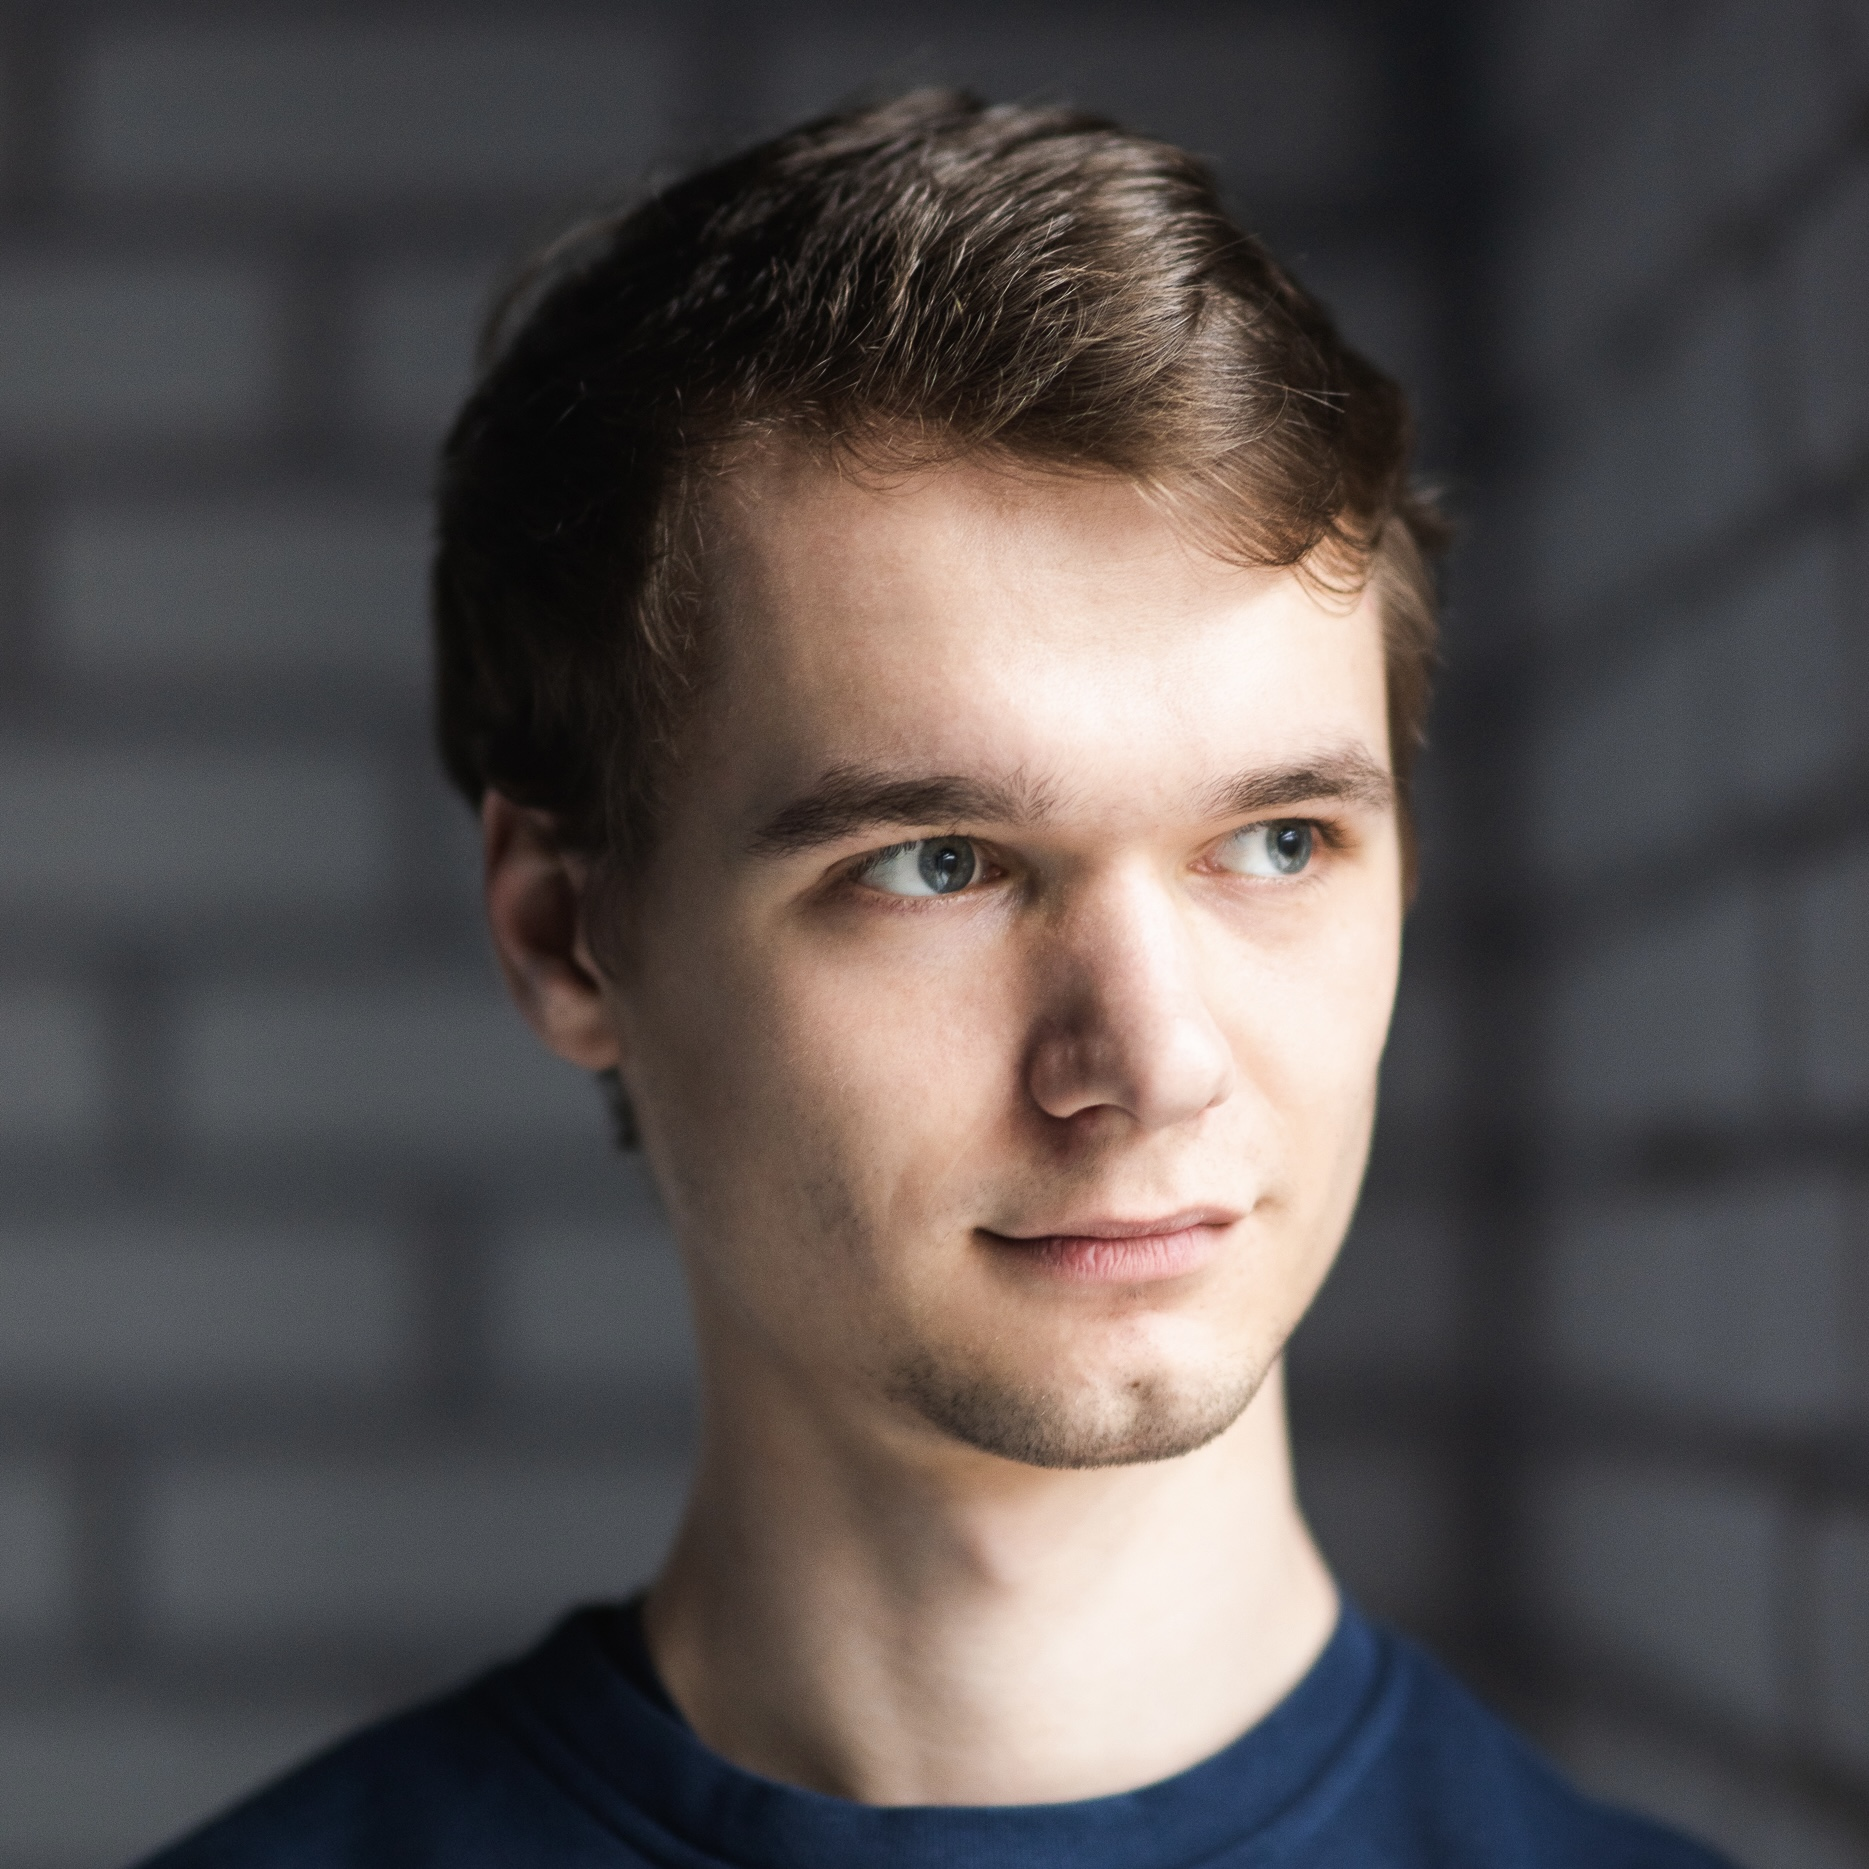
\includegraphics[width=0.62\textwidth]{me.jpg}\hfill\null

\vspace*{0.4ex}

\headleft{About me}
Former theatre and film actor who transitioned into software development through technical education and project-based work. I now focus on practical problem solving in C, C++, and Python, while bringing communication skills, discipline, adaptability, and experience working in demanding team environments.

\headleft{Contact}
\small
\MVAt\ \href{mailto:peta.simcak@gmail.com}{peta.simcak@gmail.com} \\[0.4ex]
\Mobilefone\ +420\,601\,381\,619 \\[0.4ex]
\Mundus\ \href{https://simcak.github.io}{simcak.github.io} \\[0.4ex]
\Letter\ Prague, Czech Republic \\[0.4ex]
\faGithub\ \href{https://github.com/simcak}{github.com/simcak} \\[0.4ex]
\faLinkedin\ \href{https://www.linkedin.com/in/petr-simcak}{linkedin.com/in/petr-simcak}
\normalsize

\headleft{Technical skills}
\begin{itemize}
\item C, C++, Python, Bash, MATLAB
\item Git, Docker, Linux, Nginx, LaTeX
\item Systems programming, networking, parsing
\item Backend development, signal processing
\end{itemize}

\headleft{Languages}
Czech~(C2) \\
English~(C1) \\
German~(B1)

\headleft{Highlights}
\small
2nd place at \v{S}koda Hackathon (team lead / backend role) \\[0.4ex]
Tutor at 42 Prague \\[0.4ex]
3D printer assembly, maintenance, and support
\normalsize

\end{minipage}
\kern0.08
\textwidth
}
\end{minipage}
\hskip2.2em
\begin{minipage}[t]{0.57\textwidth}
\setlength{\parskip}{0.55ex}

\vspace{1.5ex}

\headright{Selected projects}

\dates{2026--ongoing} \\
\textsc{ft\_transcendence} \textit{(full-stack web application)} \\
\smaller{Team-based web application developed at 42; current long-term project in a larger collaborative setting.}

\is
\dates{2026} \\
\textsc{ft\_irc} \textit{(C++98, sockets, poll)} \\
\smaller{Built a minimal multi-client IRC server in a team of three; worked mainly on server-side structure and IRC commands.}

\is
\dates{2025} \\
\textsc{Cub3D} \textit{(C, MLX42)} \\
\smaller{Simplified Wolfenstein-style raycasting engine; implemented parsing and core raycasting logic.}

\is
\dates{2025} \\
\textsc{Bachelor Thesis: Heart Rate Estimation from PPG Signals} \textit{(Python, signal processing)} \\
\smaller{Compared multiple methods for heart-rate estimation from physiological signals and worked on automatic signal-quality assessment.}

\is
\dates{2024--2025} \\
\textsc{Additional 42 projects} \textit{(C, Docker)} \\
\smaller{Completed minishell and Inception; gained experience with Unix processes, shell logic, containerization, and deployment setup.}

\headright{Education}

\dates{2023--2026} \\
\textsc{42 Prague} \textit{(with period at 42 Heilbronn, 2024--2025)} \\
\smaller{Software engineering curriculum based on project work, peer learning, and practical problem solving.}

\is
\dates{2020--2025} \\
\textsc{Brno University of Technology} \\
\smaller{Bachelor's Degree in Sport Technology. Thesis: \textit{Heart Rate Estimation from the PPG Signals}.}

\headright{Additional experience}

\dates{2025} \\
\textsc{\v{S}koda B3R Brigade} \textit{--- Team Lead / Backend Developer} \\
\smaller{2nd place at \v{S}koda Hackathon for a talent-matching application built with FastAPI, React, Docker, and SQLite.}

\is
\dates{2026--present} \\
\textsc{Tutor at 42 Prague} \\
\smaller{Support other students in understanding projects, debugging issues, and improving problem-solving approaches.}

\is
\dates{2022--present} \\
\textsc{3D Printer Maintenance and Support} \\
\smaller{Assembled a 3D printer at BUT and later maintained and supported its operation at 42 Prague.}

\is
\dates{2013--2021} \\
\textsc{Movie Actor} \textit{(\href{https://www.imdb.com/name/nm5791331/}{IMDb})} \\
\smaller{Worked in long-term collaborative productions in demanding environments.}

\is
\dates{2009--2015} \\
\textsc{Theatre Actor} \textit{(\href{https://www.mdb.cz/cs/lide/petr-simcak}{Brno City Theatre})} \\
\smaller{Professional stage experience in ensemble-based productions.}

\end{minipage}

\end{document}